% vim: ft=tex
\chapter{Project monitoring}
\section{Performance analysis}
% TODO checklist item: each up to 4h <--  project plan is the better place for this definition
\subsection{Weekly overview}

\autoref{fig:projmon:weekly} illustrates the weekly time spent on this bachelor
thesis. The thick horizontal line represents the planned effort of 28.5 hours a
week, which has been calculated using the risk analysis explained
in~\autoref{sec:projplan:est-time}.  Milestones are denoted by the green
labels. The legend along the x-axis represents the semester weeks, including
the particular RUP phases.


\begin{figure}[]
	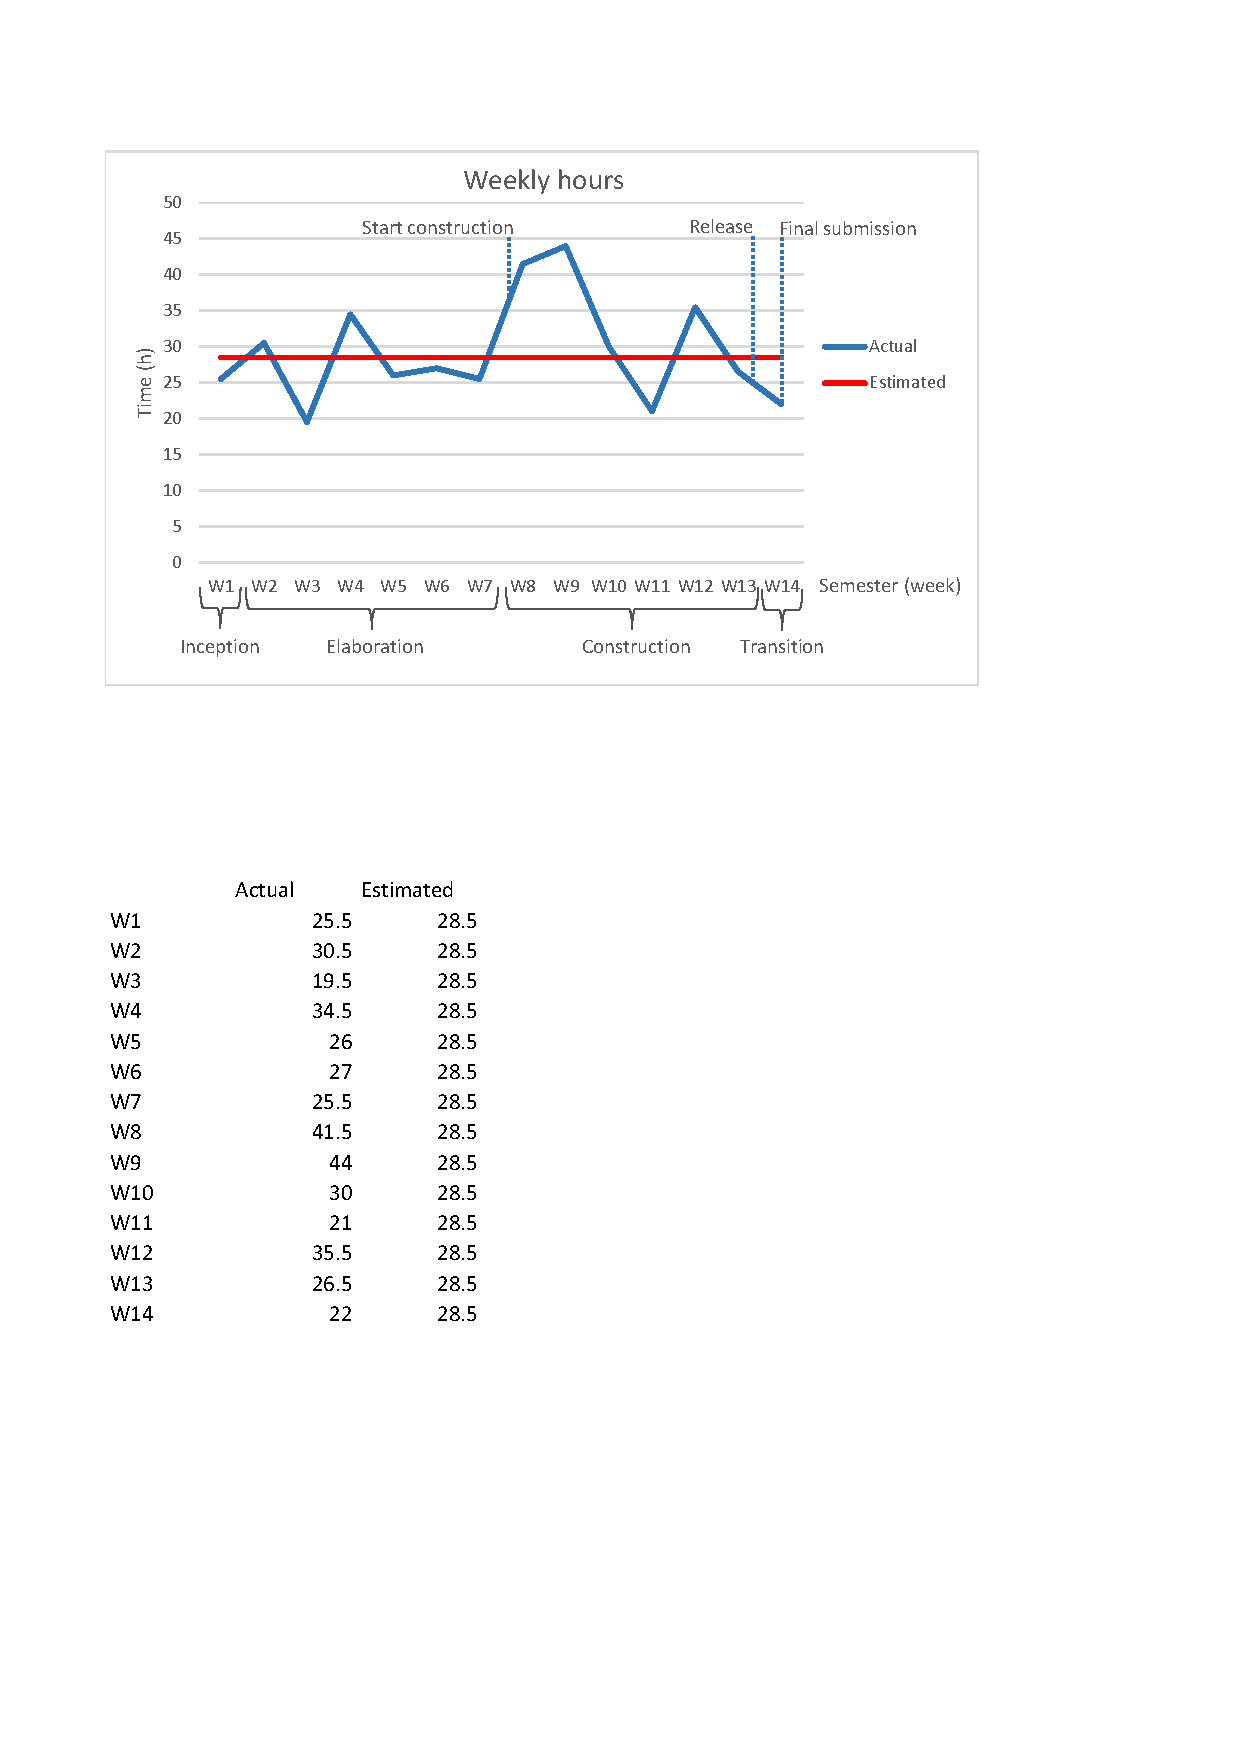
\includegraphics[trim=2cm 18.3cm 4.6cm 2.8cm, clip=true, width=\textwidth]{img/project_monitoring_weekly_hours_diagram.pdf}
	\caption{Weekly hours}
	\label{fig:weekly:hours}
\end{figure}

\begin{figure}[]
	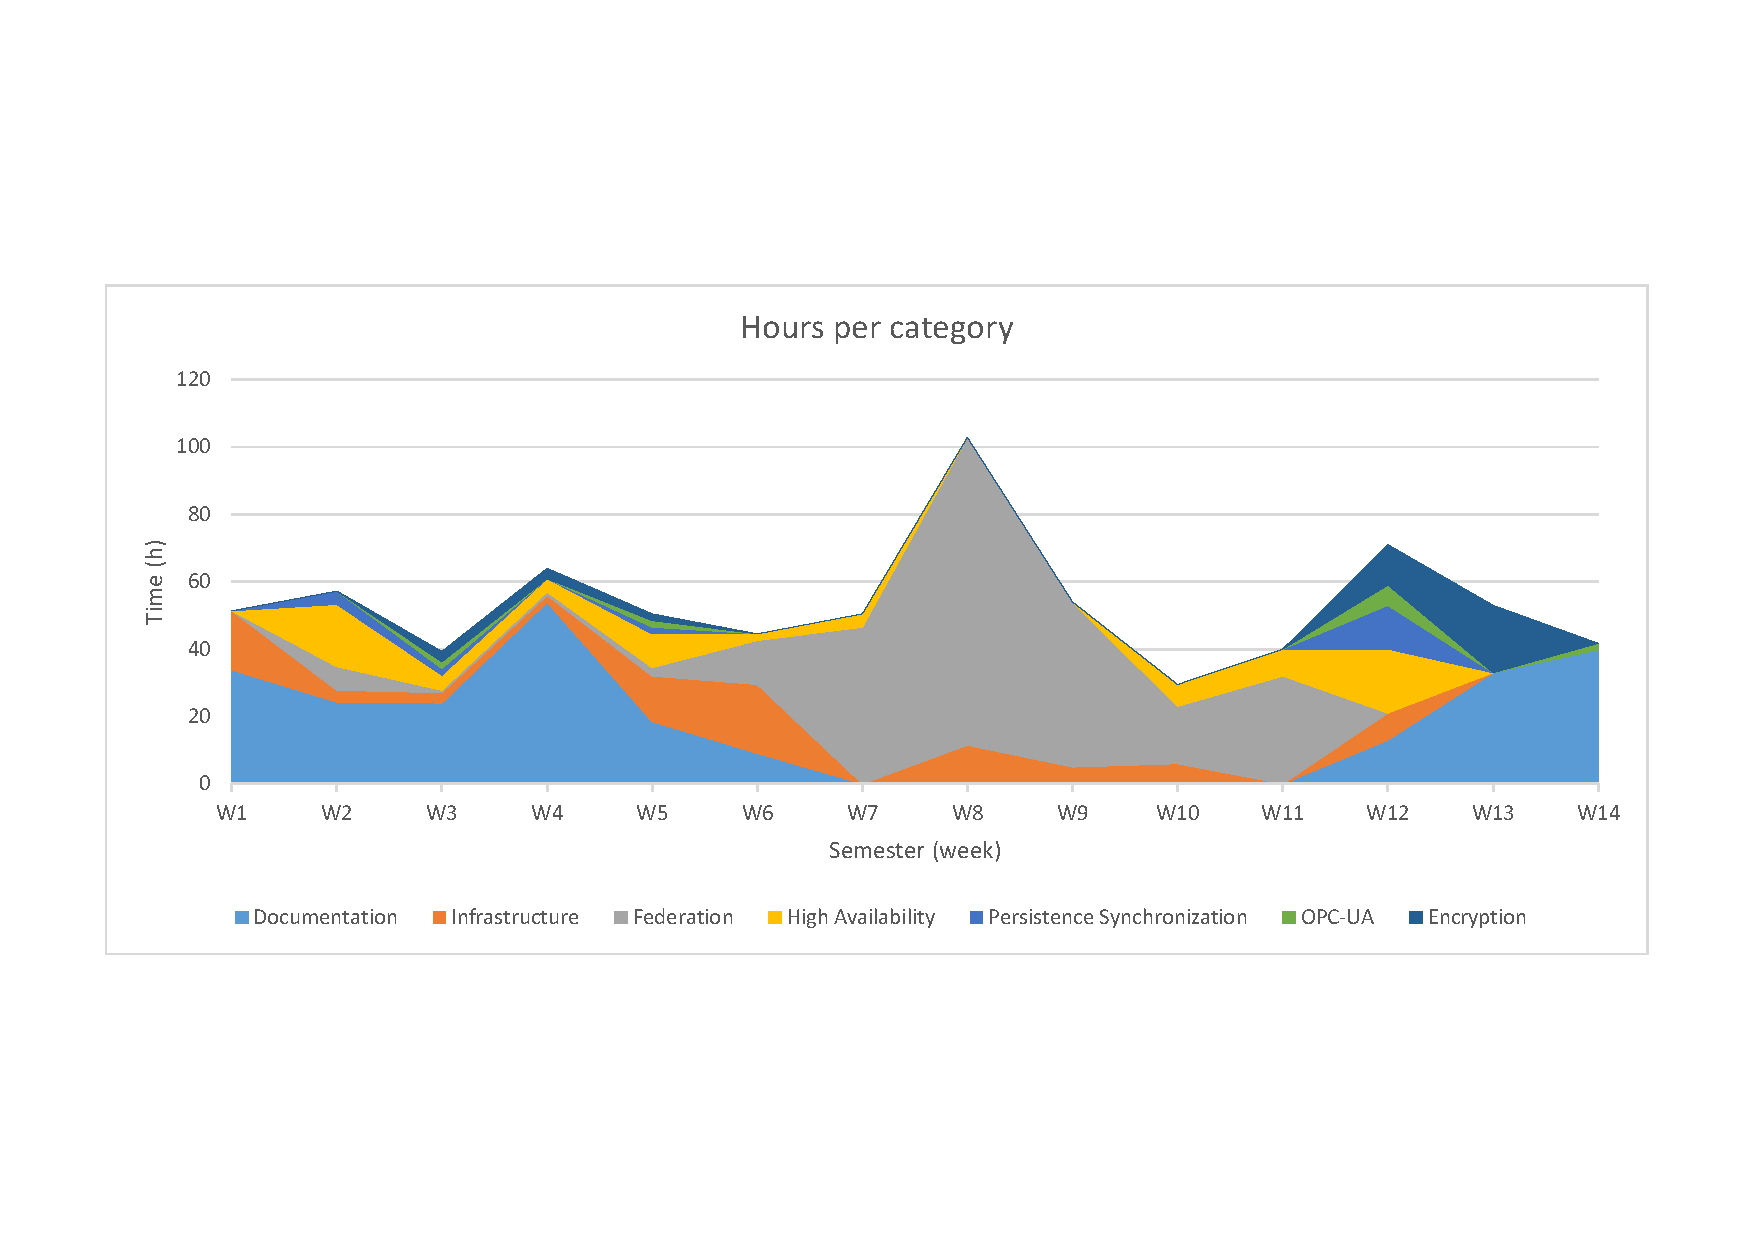
\includegraphics[trim=2cm 5cm 2cm 5.9cm, clip=true, width=\textwidth]{img/project_monitoring_weekly_hours_per_category.pdf}
	\caption{Hours per category}
	\label{fig:hours:per:category}
\end{figure}

% TODO Translate
Wie man aus dieser Grafik herauslesen kann, haben wir zu Beginn der Arbeit 
am wenigsten Stunden pro Woche aufgewendet. Das liegt daran, dass wir zuerst die 
genauen Anforderungen abklären mussten und teilweise erst nach einer Besprechung 
oder einer Rückmeldung an bestimmten Punkten weiterarbeiten konnten. 
Vor dem Meilenstein „Elaboration“ hatten wir alle Informationen zusammen und 
konnten mit vollem Elan die Anforderungen umsetzen.

As you can see from the graphic we have at the beginning of the work
the least meassured hours per week. This is because we had first to define exact requirements to be clarified and only after the kick off discussion
with the client and some of his feedbacks we could work on certain points.
Before the milestone "Elaboration" we had all the information together and
we were able to fully implement the requirements.


\begin{table}[H]
  \centering
  \begin{tabular}{|p{100mm}|p{35mm}|}
    \hline 	\bf Planned HSR hours & 720h \\ \hline
	\bf Estimated hours & 816h \\ \hline
	\bf P. Wenger worked hours & 413h \\ \hline
	\bf M. Schuler worked hours & 403h \\ \hline
	\bf Everhour tags & 14 \\ \hline
	\bf Github issues & 94 \\ \hline
	\bf Github tasks & 230 \\ \hline
	\bf Biggest issue \#33 Refine Document & 80h \\ \hline
  \end{tabular} \\
  \caption{Project statistics}
  \label{tab:projectstats}
\end{table}


% TODO translate
Die von der Modulbeschreibung geforderten, Soll-Stunden wurden um 10% überschritten haben. 
Der Grund der Überschreitung ist unteranderem
die Implementation der optionalen Features und das ersten Feature CSP brauchte mehr Zeit als geplant. Es wurde während der Prototyp Phase
festgestellt das es eventuell mehr Zeit benötigten wird als eingeplant in die Einarbeitung von Roadster. 
Grund dafür war das fehlende Wissen und die "Perfektionswut".
Im weiteren Projektverlauf konnte die Performance der einzelnen Projektmitarbeiter gesteigert werden
was auf das erlernte Wissen über Roadster zurückzuführen war, sowie durch die gut
Strukturiere Architektur von Roadster was uns das Erweitern der Software sichtlich erleichtert hat.

Die einzelnen Personen haben ein sehr ausgeglichenes Stundentotal. 
Das liegt daran, dass wir in regelmässigen Abständen eine Auswertung 
in Everhour gemacht haben und dadurch die Tasks gerechter verteilen konnten. 

The nominal hours required by the module description have exceeded over 10%.
One of the reason for the overshoot is among others the implementation of the optional features and the first feature took more time than planned. 
During the prototype phase we found out that it took eventually more time than planned in the learning process of Roadster. The missing knowledge and
The "perfection rage" was for another reason.
After the implementation of the CSP feature we could improve our efficency and henceforth everything seems to work adhoc.

The individual persons have a very balanced hours total, because we had an evaluation at regular intervals
in Everhour and thereby distribute the tasks more equitably.


\subsection{Aufgewendete Stunden nach Feature}
% TODO Translate
Da wir in dieser Arbeit ein bestehendes Produkt erweitert haben war es zu beginn an
schwierig die Aufwände abzuschätzen. Die Soll/Ist Abschätzungen wurden von Iteration zu Iteration
immer genauer. Nachfolgend die Soll/Ist Aufwandschätzung der einzelnen Feature.

At beginning it was hard to asses the estimated hours of the first feature. After each iteration our estimation planning
became more accurate that's why we could achieve the final submission without any rush. This followed graphic shows it perfectly:

\begin{figure}[]
	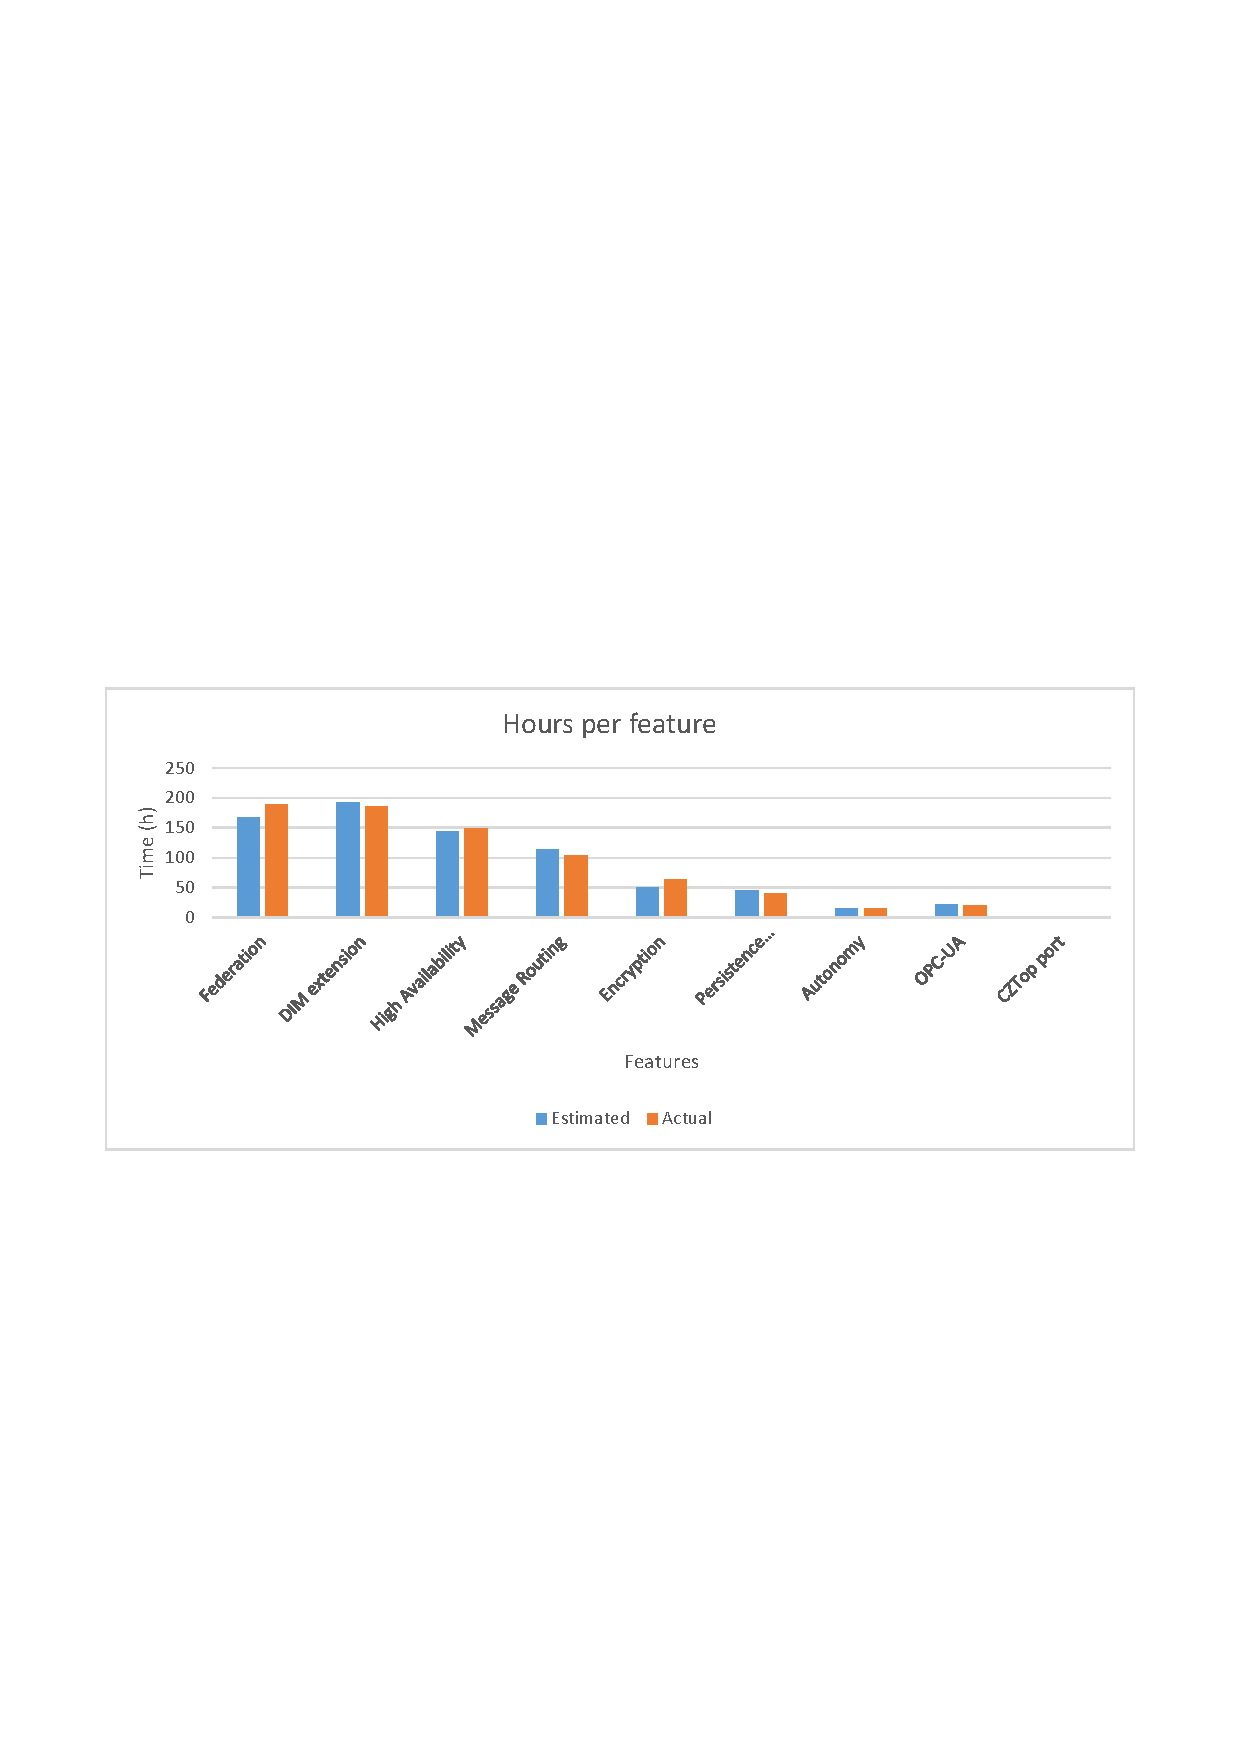
\includegraphics[trim=2cm 10.5cm 2cm 11.9cm, clip=true, width=\textwidth]{img/project_monitoring_hours_per_feature_diagram.pdf}
	\caption{Hours per feature}
	\label{fig:hours:per:feature}
\end{figure}


% TODO translate
Die Archivdaten unseres Everhour Projekts befinden sich auf dem Moodle. 
In diesem kann detailliert nachverfolgt werden, 
für welche Tasks wir wie viel Zeit aufgewendet haben.

The archive data from everhour project can be found on moodle. Everything can be derived from these data.

\subsection{Effort by activity}
% TODO category diagram
\begin{figure}[]
	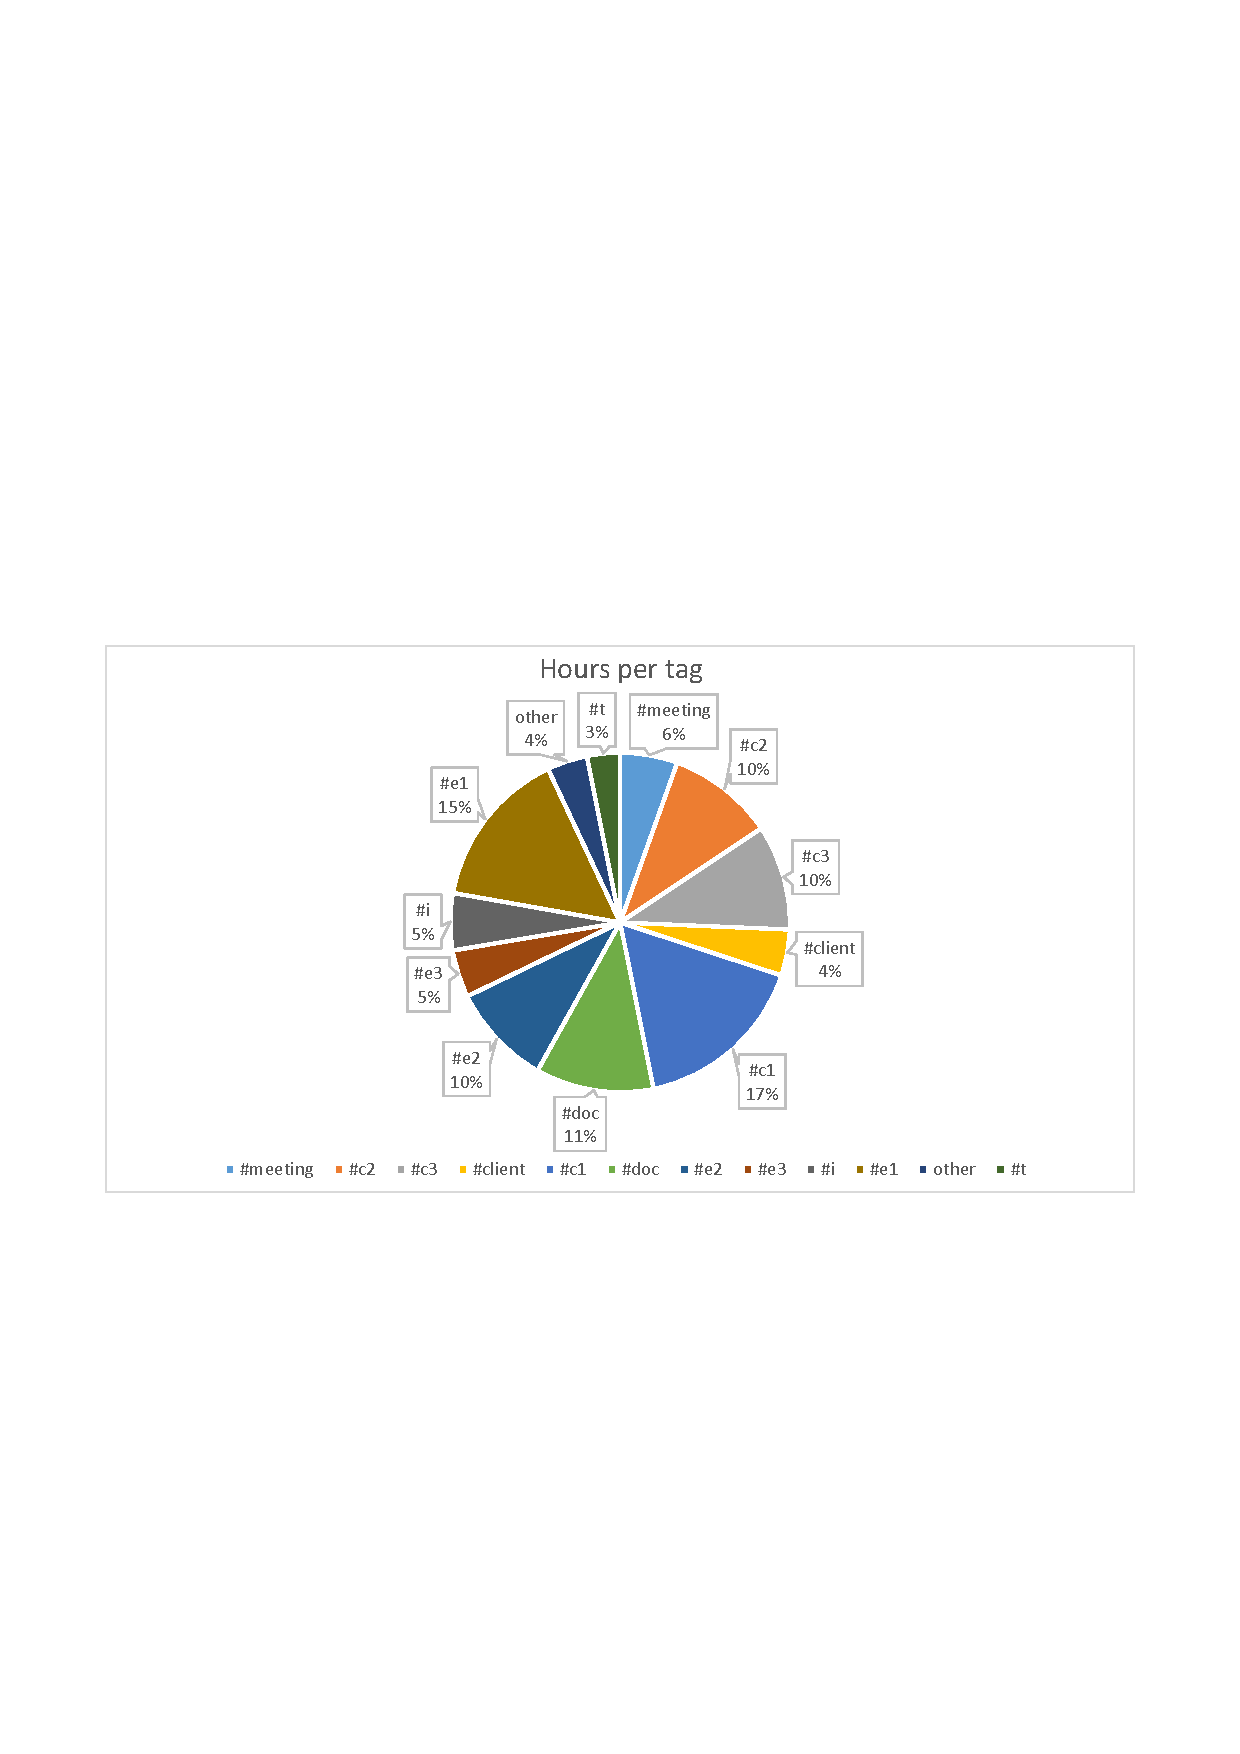
\includegraphics[trim=4cm 9.6cm 3.5cm 11.1cm, clip=true, width=\textwidth]{img/project_monitoring_hours_per_tag_diagram.pdf}
	\caption{Hours per tag}
	\label{fig:hours:per:tag}
\end{figure}

8\% der ganzen Projektdauer wurde für Projektmanagement
und Meetings aufgewendet. 2\% davon sind für Requirements besprechung mit dem Kunden. Die Verteilung
entspricht vollumfänglich der geplanten Phasen. 

8\% from the whole project duration was for project management and meetings. 2\% was for requirements meetings with the client.
The distribution corresponds fully to the planned phases.
